%This is a LaTeX file for producing Adobe portable
%document files suitable for AMS extended abstracts.
%	Christopher M. Godfrey
%	University of North Carolina Asheville
%
%%%%%%%%%%%%%%%%%%%%%%%%%%%%%%%%%%%%%%%%%%%%%%%%%%
\documentclass[twocolumn]{article}

\usepackage{preprint}	%Use style file 'preprint.sty'
\usepackage{epsfig}		%Use postscript (.eps Figures)
\usepackage{indentfirst}%Indent the first paragraph in each section
\usepackage{graphicx}	%Allows \includegraphics
\usepackage{epic}		%Allows picture
\usepackage{eepic} 		%Allows more commands to work in picture
\usepackage{float} 		%Allows use of [H] option on floats
\usepackage{textcomp}	%Makes special symbols where necessary (need 'textcomp.sty')
\usepackage{amsmath}	%Adjusts size of delimiters in equations
\usepackage{url}		%Allows a proper looking URL format
\urlstyle{same}


%Use this if you're brave and want multiple columns - beware of float problems!
%\usepackage{multicol}

\graphicspath{{./Figures/}}	%Store figures separately

%Change the way figures are labeled
\renewcommand{\figurename}{\textsc{Fig.}}

%Change the way tables are labeled
\renewcommand{\tablename}{\textsc{Table}}

%Change the font in captions to make text smaller
\newcommand{\captionfonts}{\footnotesize}

%Modify caption styles to match AMS format
\makeatletter  % Allow the use of @ in command names
\long\def\@makecaption#1#2{%
  %\vskip\abovecaptionskip	%Adds extra space below a figure/before a caption
  \sbox\@tempboxa{{\captionfonts #1. #2}}%
  \ifdim \wd\@tempboxa >\hsize
    {\captionfonts #1. #2\par}
  \else
    \hbox to\hsize{\hfil\box\@tempboxa\hfil}%
  \fi
  \vskip\belowcaptionskip}
\makeatother   % Cancel the effect of \makeatletter

%Fix floats in multicolumn environment - also works with 'twocolumn' class
\makeatletter
\newenvironment{tablehere}
  {\def\@captype{table}}
  {}
\newenvironment{figurehere}
  {\def\@captype{figure}}
  {}
\makeatother

%Uncomment to center the last line of captions
%\usepackage{ccaption}
%\captionstyle{\centerlastline}

%%%%%%%%%%%%%%%%%%%%%%%%%%%%%%%%%%%%%%%%%%%%%%%%%%
%Start article here
\begin{document}

%Span both columns
\twocolumn[%

%Insert small space at top of title page
\vspace{0.125in}

%Insert the paper number
{\textbf{
%%%My paper number is...>>>>>>>>>>
Pressure Analysis
%%%<<<<<<<<<<<<<<<<<<<<<<<<<<<<<<<
}}

%Bring the title back up to the same line as the paper number
%%%>>>>>>>>>>UNCOMMENT ONE>>>>>>>>
%\vspace{-0.39in}	%My title is large
\vspace{-0.235in}	%My title is small
%%%<<<<<<<<<<<<<<<<<<<<<<<<<<<<<<<

%Make the title
\begin{center}
\setstretch{1.3}	%Sets title line spacing

%%%>>>>>>>>>>UNCOMMENT ONE>>>>>>>>
%{\textbf{\large{	%My title is large/bold
%{{\large{			%My title is large/not bold
{\textbf{{			%My title is small/bold
%{{{				%My title is small/not bold
%%%Title>>>>>>>>>>>>>>>>
MEASUREMENTS OF LOCAL PRESSURE AND HEIGHT USING RAW DATA TO FIND SCALE HEIGHT
%%%<<<<<<<<<<<<<<<<<<<<<
}}}
\end{center}
\begin{center}
%%%First Author>>>>>>>>>>>>>>>
Douglas J. March$^{*}$
%%%<<<<<<<<<<<<<<<<<<<<<
\\
%%%Affiliation>>>>>>>>>>
University of North Carolina - Asheville\\
%%%<<<<<<<<<<<<<<<<<<<<<
\vspace{3mm}
\end{center}

]	%You need this bracket!

%Create the corresponding author footnote
{\textfloatsep 0.1875in
\begin{table}[!b]
\hrule height 0.05pt width 0.5625in	%Horizontal line
\vspace{0.125in}
\setstretch{0.76}	%Adjust line spacing
{\footnotesize
%\hspace{2mm}		%No indent for preprints
{\it $^{*}$Corresponding author address:}
%>>>>>>>>>PLACE CORRESPONDING AUTHOR HERE>>>>>>>>>>>>>>>
Douglas J. March, University of North Carolina - Asheville, 
Someplace in Asheville, Asheville, North Carolina 28805; e-mail:
dmarch@unca.edu
%<<<<<<<<<<<<<<<<<<<<<<<<<<<<<<<<<<<<<<<<<<<<<<<<<<<<<<<
%Use "\\" above to break the line between postal and email addresses (non-preprint)
}
\end{table}
}

%PLACE TEXT OF ARTICLE HERE>>>>
\section{{\normalsize \hspace{-0.195in} {\textbf{
%%%Insert section heading below>>>>>>>>>>>>
INTRODUCTION
%%%<<<<<<<<<<<<<<<<<<<<<<<<<<<<<<<<<<<<<<<<
}}}} \vspace{-1.6mm}
\label{pres_intro.sec}
Air pressure is essential to life on Earth as we know it. Its importance ranges from the conditions of the skies to the amount of gas absorption in water. At higher elevations, gases, like oxygen, cannot dissolve as readily into water than at lower elevations because of the lack of atmospheric pressure needed for the solution to absorb the gas. Also, atmospheric pressure can cause the skies to be clear and sunny or cloudy and rainy. Depending on which side of the high pressure cell one is located, the higher pressure means a more stable atmosphere, thus causing less clouds to appear and a higher diurnal temperature range. When the pressure becomes low, the atmosphere becomes unstable causing clouds to form and precipitation to fall.

This experiment used two pressure measurements and two elevation readings, one from the top of Purchase Knob and another from the base of the mountain to estimate the atmospheric pressure changes with distance in the vertical and horizontal directions. Raw Kestrel surface pressure data and the true surface pressure data at the UNCA campus were used to calibrate the pressure readings. All these measurements and calculations determined the scale height and how quickly it changes with height. 
 
\section{{\normalsize \hspace{-0.195in} {\textbf{
%%%Insert section heading below>>>>>>>>>>>>
METHODOLOGY
%%%<<<<<<<<<<<<<<<<<<<<<<<<<<<<<<<<<<<<<<<<
}}}} \vspace{-1.6mm}
\label{pres_method.sec}

The objective was to analyze the pressure and height readings given at the Purchase Knob Research Center, calibrate them with the real data given at the UNCA campus, and determine the scale height using the highest elevation data point.\\
The equipment that was used:\\
-	(1) Personal Computer\\
-	(1) Kestrel 4000 NK\\
-	(2) Garmin eTrex – Vista CX\\
The measurements of pressure were taken with the Kestrel and the elevation with the Garmins at the base of Purchase Knob and again at the Purchase Knob Research Center near the top. For each location, the Kestrel was used to determine the pressure measurements and the Garmins to determine the elevation. This data was used with the formulas to estimate the atmospheric scale height from the two given locations. 
The scale height $H$ (m) was determined by using equation~\ref{pres:qg} and the measurements taken from table~\ref{presdata}. For $H$ (m), the numerator $A$ was found by computing $z-z_B$ as $1476-786=690$, and the denominator $B$ was found by computing $\ln{p(z)}-\ln{(p(z_B)}$ as $\ln{850}-\ln{924.75}=0.08483$. With both $A$ and $B$ determined, division of $\frac{A}{B}*(-1)$ gave a final height $=8186.3079$ (m). Since $H$ (m) was now determined, equation~\ref{pres:cg} could be used to determine the air pressure $p$ (hPa) at an altitude $z$ (m). The numerator was the same one used in equation~\ref{pres:qg} with a $(*-1)$ and the denominator was the solution to $B$. This was used in the final equation $924.75\exp^{\frac{A*(-1)}{B}} = 701.49$ (hPa).
%Use \displaystyle to make a fraction or exponent match the regular size of the text here. 
Formulas used:
\begin{equation}\label{pres:cg}
p(z)=p(z_B)exp({-\frac{z-z_B}{H}-z_B)},
\end{equation}
where $p$ is pressure (hPa), $z$ is the elevation at given locations (m), $z_B$ is base location, $H$ is  the scale height (m)

\begin{equation}\label{pres:qg}
H={-\frac{z-z_B}{\ln{p(z)}-\ln{p(z_B)}}},
\end{equation}

where $H$ is the scale height (m), where $p$ is pressure (hPa), $z$ is the elevation at given locations (m), $z_B$ is base elevation.

\section{{\normalsize \hspace{-0.195in} {\textbf{
%%%Insert section heading below>>>>>>>>>>>>
DATA
%%%<<<<<<<<<<<<<<<<<<<<<<<<<<<<<<<<<<<<<<<<
}}}} \vspace{-1.6mm}

\begin{table}[t!] %[!htbp]
\centering
\caption{
\\The results of the pressure and altitude at both locations. (Note: All of the pressure measurements have been corrected by a factor of +1 hPa)}
\label{presdata}
\begin{tabular}{|l||c|r|}
\hline
Location &  Altitude & Pressure\\
\hline \hline
Purchase Knob Top & 1476 m & 850 hPa\\
\hline
Purchase Knob Base & 786 m & 924.75 hPa\\
\hline
\end{tabular}
%\end{center}
\end{table}
\\

%
\begin{figure}[!t] %[!htbp]
\begin{center}
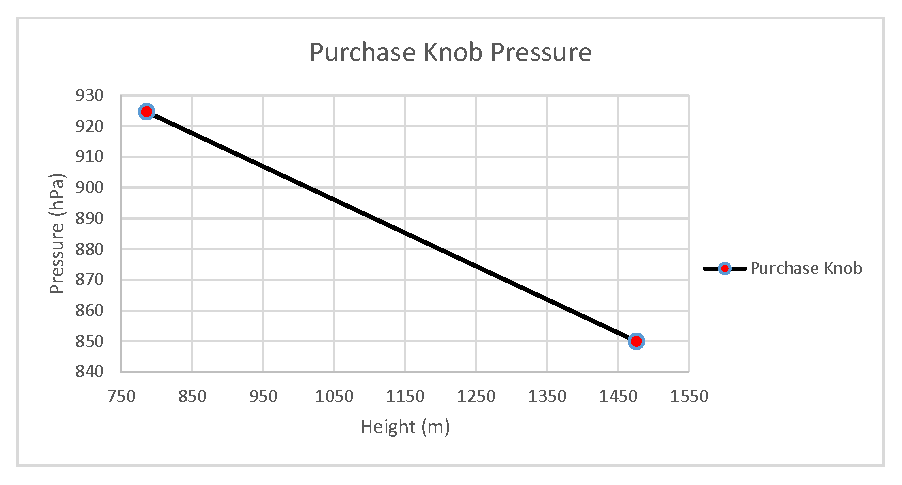
\includegraphics[angle=0, width=0.48\textwidth]{PurchaseKnob}
\end{center}
\caption{
Purchase Knob change in pressure from the base of the mountain to the top.
\label{Pknob}
}
\end{figure}
%


The results in Table~\ref{presdata} are raw measurements with the Kestrel and properly calibrated using measurements from the rooftop station at UNCA. There was a difference of +1 hPa between the two devices and I compensated for this by adding the difference to the raw data results. My results indicate that there was a strong pressure difference between the bottom of the mountain and the top, and when calculated, the scale height is slightly above average at 8186.3 m where the average is 7640 m.

A potential error in forecasting surface pressure and vertical pressure change is a miscalibration in the instruments used to acquire the raw data. Without a properly calibrated instrument, the pressure readings may be skewed causing an incorrect measurement of the vertical pressure changes after calculations are done.

Another potential error in forecasting the horizontal and vertical pressure changes may be a quick moving supercell system that brings with it a very rapid decrease in pressure. This error can be resolved by just visual observation out in the field or by reviewing the radar data. If a supercell were to pass over the instrument, one could observe and calculate a very large increase in the scale height due to drastic instability in atmospheric pressure and strong surface convergence. This data is supported by looking at Figure ~\ref{map} and noting that while the pressure may be stable across the region, if a supercell moved over a weather station then these results could be skewed.

%%%%%%%%%%%%%%%%%%%%%%%%%%%%%%%%%%%%%%%%%%%%%%%%%%%%%%%%%%%%%%%%%%%%
\begin{figure}[!t] %[!htbp]
\begin{center}
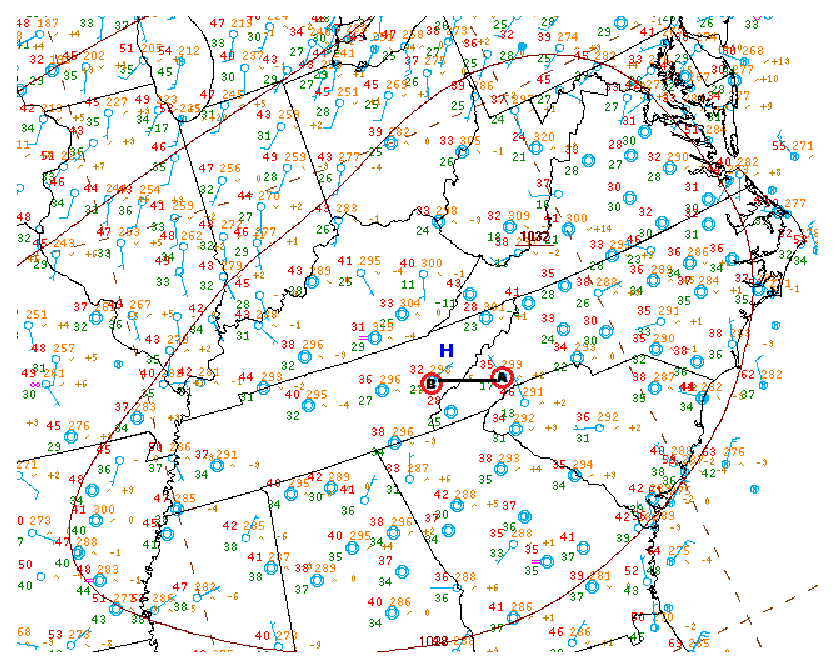
\includegraphics[angle=0, width=0.48\textwidth]{map}
\end{center}
\caption{
The SLP map shows two points (A , B) at a distance of 95 km apart.
\label{map}
}
\end{figure}
%%%%%%%%%%%%%%%%%%%%%%%%%%%%%%%%%%%%%%%%%%%%%%%%%%%%%%%%%%%%%%%%%%%%
\section{{\normalsize \hspace{-0.195in} {\textbf{
%%%Insert section heading below>>>>>>>>>>>>
EXTENSION QUESTIONS
%%%<<<<<<<<<<<<<<<<<<<<<<<<<<<<<<<<<<<<<<<<
}}}} \vspace{-1.6mm}
\label{presure_extques.sec}

\underline{Q1}: Use your exponential function for pressure to estimate the pressure at an altitude of [1] 3800 feet and [2] 7000 feet. What might be the difference in using this expression to estimate the pressure at the different elevations (hint: note the difference in interpolation v. extrapolation)?

\underline{A}: If I used formula 1 to estimate the pressure at an altitude of 1158.24 m and 2133.6 m, the air pressure would be 883.642 hPa and 784.391 hPa respectively. The difference in using this expression to estimate the pressure at these different elevations would be the known height of $z$, where $z_B$, scale height $H$, and pressure at $z_B$ all remain constant. \\

\underline{Q2}: How would the scale height $H$ in the expression above change if the air temperature on the day of the measurements was much hotter than what was observed?

\underline{A}: If the air temperature on the day of the measurements were much hotter than what was previously observed, then the scale height $H$ in the question above would increase. This is because hotter temperatures would indicate the change in air pressure aloft (from the previous question) would decrease with height less rapidly since hotter air rises and expands. Since scale height is a way to represent how pressure values decrease with height by a factor of  $1/e$, the rate of change in a hotter vertical profile of air pressure would also decrease. \\

\underline{Q3}: Find a sea level pressure map with isobars plotted for a region near Asheville. Calculate how much the pressure changes from Asheville in a straight line to the Tennessee/NC border (about 45 kilometers). What is the estimated pressure change using your exponential function of pressure if you ascended to an altitude of 45 kilometers? Given the two calculations in Question 3, what can you say about how atmospheric pressure changes over a given distance in the horizontal direction compared with its change over the same distance in a vertical direction?

\underline{A}: As seen in Figure~\ref{map}, If I calculated the pressure change in a straight line from point A, where the pressure is 1029.9 hPa, to point B, where the pressure is 1029.8 then there would only be a change of -0.1 hPa. If these locations are 90 km apart and the boarder of Tennessee is 45 km from point A then there is an estimated change of only -0.05 hPa. However, if the measurement was not made horizontally but vertically, the pressure would fall to 4.647 hPa at an elevation of 45 km. Comparing the two measurements gives an idea of just how quickly pressure can fall. If one were to drive their car for an hour at a horizontal distance of 45 km from where they started, there would be a very minimal change in atmospheric pressure, but if it were possible to drive a car vertically for an hour at a distance of 45 km, the person would asphyxiate quite quickly due to a lack of atmospheric pressure. 

%%%%%%%%%%%%%%%%%%%%%%%%%%%%%%%%%%%%%%%%%%%%%%%%%%%%%%%%%%%%%%%%%%%%%

\section{{\normalsize \hspace{-0.195in} {\textbf{
%%%Insert section heading below>>>>>>>>>>>>
CONCLUSIONS
%%%<<<<<<<<<<<<<<<<<<<<<<<<<<<<<<<<<<<<<<<<
}}}} \vspace{-1.6mm}
\label{etacomp_conc.sec}

Through the analysis of data measured between the two locations, there is now a better understanding of the measurements used in determining how pressure changes with altitude in both horizontal and vertical distances. 

A large factor in determining pressure is temperature. This may cause the scale height to increase where the pressure profile doesn’t increase as rapidly as if there was a divergence aloft – when cold surface air is converging, lowering the scale height. A strong vertical wind shear may also effect the pressure, where strong winds aloft can bring in colder air, increasing the surface temperature and pressure resulting in a decreased scale height.

Another factor would be the time of day that the measurements are taken at. Early in the morning the surface tends to be cooler and the atmosphere more stable causing a decreased scale height, unlike in the afternoon when the atmosphere becomes unstable and the scale height increases due to warmer air aloft. Also, the horizontal distance between two places may change the scale height for any given location, for example, cold air damming along the Appalachian Mountains can cause drastic pressure differences between two cities located on opposite sides of the ridge. This pressure difference may result in radical differences in scale height for each city. $\bullet$ 

%END TEXT OF ARTICLE<<<<<<<<<<<

%\begin{acknowledgments}

%\end{acknowledgments}

%You could use BibTeX to create citations instead...

\begin{references}
%\begin{thebibliography}{3} %%Use with \bibitem

{\footnotesize
%
\item{Ahrens} 
Ahrens, C. Donald, 2012: Essentials of Meteorology: An Invitation to the Atmosphere.
\textit{Brooks/Cole Cengage Learning}
\textbf{109,} 506 pp.

%\vspace{0.235mm}

\item{Harvard}
Harvard University, 2014: Atmospheric Chemistry Modeling Group. Accessed 15 November 2015. 
\textbf{11,} Available online at 
\\\url{[http://acmg.seas.harvard.edu/people/faculty/djj/book/bookchap2.html]}

%Using \vspace between references on the last page is a simple way to balance
%the columns within an environment where something like the package balance.sty
%won't do the trick.
%\vspace{0.235mm}

\item{NOAA} 
NOAA, 2015: Weather Prediction Center \& Archived Data. Accessed 15 November 2015.
\textbf{109,} Available online at
\\\url{[http://www.wpc.ncep.noaa.gov/html/sfczoom.php?h=15&y=2015&m= 11&d=15]}


%\vspace{0.235mm}


}	%End footnotesize
\end{references}
%\end{thebibliography}

\end{document}
